 \documentclass{article}
 
\usepackage[
	colorlinks,
	urlcolor={blue}
]{hyperref}
\usepackage{tikz}
\usetikzlibrary{arrows.meta}
 
\title{Supplement for ``Ordering Induction''}
\author{Julian Zucker, julian.zucker@gmail.com}
\date{}

\begin{document}
\maketitle

\section{Background}
When trying to do analysis on the dataset mentioned in the abstract, I ran into an issue -- there are no methods for applying ordering-based methods such as Borda count to intransitive incomplete pairwise vote sets. Much work has been done on incomplete vote sets, but many researchers believe that having intransitive votes is irrational. While Northeastern does not have active research in social choice or computational social choice, meaning we cannot guarantee that no such thing exists in the modern literature, the professors on the project were also unable to find any algorithms for converting intransitive incomplete pairwise vote sets to orderings. So, we set out to create our own.

\subsection{The Dog Project}
The Dog Project was a undergraduate research project at Northeastern, focusing on applied social choice. We wanted to identify the cutest dog in the philosophy department, so we collected 59,052 votes from 937 voters on 26 dogs. While this project was, at least on it's face, not related to multi-agent systems, social choice theory applies equally to combining multiple human decisions into one societal decision as it does to combining multiple agent's decisions to make one overall decision.

\subsection{Open-Source Work} 
The code for ordering induction, as well as a broad selection of social choice algorithms, has been open-sourced, and is available \href{https://github.com/julian-zucker/socialchoice}{here} and \href{https://pypi.org/project/socialchoice/}{on PyPI}. The hope is to foster more open social choice research, and to allow the work that went into implementing social choice mechanisms for the dog project to not be wasted. The code and data that generated the results in the paper is available \href{https://github.com/julian-zucker/vote-induction}{here}, and reproducible by following the instructions in the README.
 

\section{Methods}
This method was only evaluated on one dataset. This seems bad, the method has not yet been shown to be robust on multiple datasets. However, the scarcity of intransitive incomplete pairwise vote sets makes it difficult to find new source material -- Preflib does not have pairwise vote sets that are both intransitive and incomplete, so the only way to find this data would be to trust some third party's data collection or run another ``election'' like the dog project. Simulation methods were considered, as creating simulations of voters and then processing their votes might give some reasonable level of confidence in the accuracy of ordering induction methods, but the additional complexity of the simulation, and the risk of simulations that don't accurately capture real voter's opinions, lead me to eschew simulations for data generation.

\subsection{Visual Explanation of Ordering Induction}
Pairwise comparisons are easily represented as directed graphs, where each edge from node $U$ to node $V$ represents $U$ being chosen over $V$ in a pairwise comparison. Imagine the following votes were made by one voter, in an election with six candidates:

\begin{center}
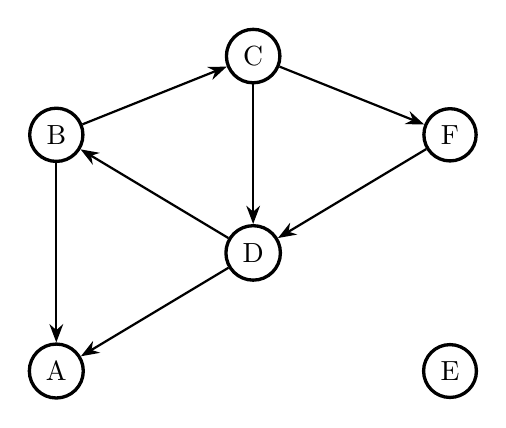
\begin{tikzpicture}
\begin{scope}[every node/.style={circle,very thick,draw}]
    \node (A) at (0,0) {A};
    \node (B) at (0,3) {B};
    \node (C) at (2.5,4) {C};
    \node (D) at (2.5,1.5) {D};
    \node (E) at (5,0) {E};
    \node (F) at (5,3) {F} ;
\end{scope}

\begin{scope}[>={Stealth[black]},
              every node/.style={fill=white,circle},
              every edge/.style={draw=black, thick}]
    \path [->] (B) edge (A);
    \path [->] (B) edge (C);
    \path [->] (D) edge (B);
    \path [->] (D) edge  (A);
    \path [->] (C) edge (D);
    \path [->] (F) edge (D);
    \path [->] (C) edge  (F);
\end{scope}
\end{tikzpicture}
\end{center}

This vote set is intransitive, because there is a cycle $(C, D, B, C)$, and incomplete, because $E$ has not been voted on. The first step that the ordering induction method must take is removing the intransitivity. Suppose that this is accomplished be removing the $(B,C)$ edge.

\begin{center}
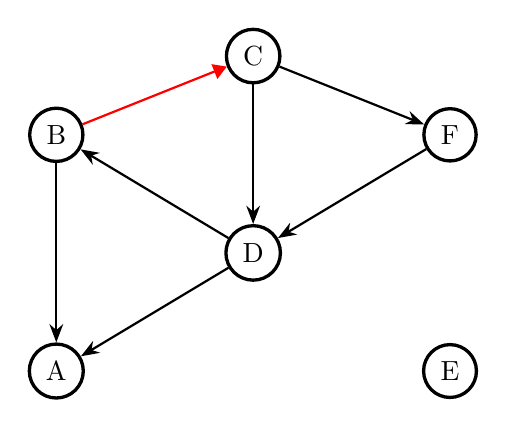
\begin{tikzpicture}
\begin{scope}[every node/.style={circle,very thick,draw}]
    \node (A) at (0,0) {A};
    \node (B) at (0,3) {B};
    \node (C) at (2.5,4) {C};
    \node (D) at (2.5,1.5) {D};
    \node (E) at (5,0) {E};
    \node (F) at (5,3) {F} ;
\end{scope}

\begin{scope}[>={Stealth[black]},
              every node/.style={fill=white,circle},
              every edge/.style={draw=black, thick}]
    \path [->] (B) edge (A);
    \path [->] (F) edge (D);
    \path [->] (D) edge (B);
    \path [->] (D) edge  (A);
    \path [->] (C) edge (D);
    \path [-{Triangle[fill=red]}] (B) edge[red] (C);
    \path [->] (C) edge  (F);
\end{scope}
\end{tikzpicture}
\end{center}

This leaves us with the following vote set:
\begin{center}
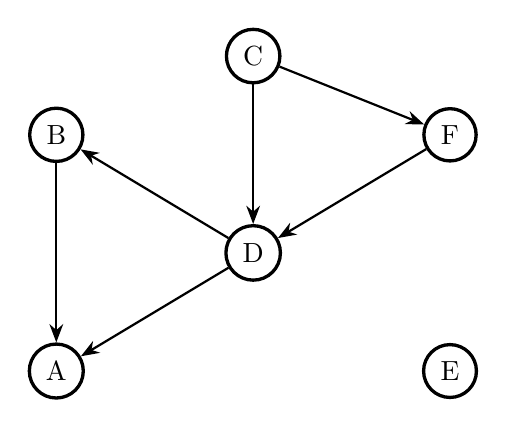
\begin{tikzpicture}
\begin{scope}[every node/.style={circle,very thick,draw}]
    \node (A) at (0,0) {A};
    \node (B) at (0,3) {B};
    \node (C) at (2.5,4) {C};
    \node (D) at (2.5,1.5) {D};
    \node (E) at (5,0) {E};
    \node (F) at (5,3) {F} ;
\end{scope}

\begin{scope}[>={Stealth[black]},
              every node/.style={fill=white,circle},
              every edge/.style={draw=black, thick}]
    \path [->] (B) edge (A);
    \path [->] (F) edge (D);
    \path [->] (D) edge (B);
    \path [->] (D) edge  (A);
    \path [->] (C) edge (D);
    \path [->] (C) edge  (F);
\end{scope}
\end{tikzpicture}
\end{center}

Now we have a transitive, albeit incomplete, vote set. At this point, the graph could be topologically sorted; however, the topological sort would be underdetermined (as there are multiple possible orders), and more damningly, not contain every node. Because there are no votes on E, it could be placed in any position within the topological sort. So, we must carry out the second step in an ordering induction method, adding edges until there is only one possible outcome.

\definecolor{darkgreen}{rgb}{.3,.7,.3}
\begin{center}
\begin{tikzpicture}
\begin{scope}[every node/.style={circle,very thick,draw}]
    \node (A) at (0,0) {A};
    \node (B) at (0,3) {B};
    \node (C) at (2.5,4) {C};
    \node (D) at (2.5,.7) {D};
    \node (E) at (5,0) {E};
    \node (F) at (5,3) {F} ;
\end{scope}

\begin{scope}[>={Stealth[black]},
              every node/.style={fill=white,circle},
              every edge/.style={draw=black, thick}]
    \path [->] (B) edge (A);
    \path [->] (F) edge (D);
    \path [->] (D) edge (B);
    \path [->] (D) edge  (A);
    \path [->] (C) edge (D);
    \path [->] (C) edge  (F);
    \path [-{Triangle[fill=darkgreen]}] (C) edge[darkgreen] (B);
    \path [-{Triangle[fill=darkgreen]}] (C) edge[darkgreen] (A);
    \path [-{Triangle[fill=darkgreen]}] (C) edge[darkgreen] (E);
    \path [-{Triangle[fill=darkgreen]}] (F) edge[darkgreen] (E);
    \path [-{Triangle[fill=darkgreen]}] (F) edge[darkgreen] (B);
    \path [-{Triangle[fill=darkgreen]}] (D) edge[darkgreen] (E);
    \path [-{Triangle[fill=darkgreen]}] (A) edge[darkgreen] (E);
    \path [-{Triangle[fill=darkgreen]}] (B) edge[darkgreen] (E);
    \path [-{Triangle[fill=darkgreen]}] (F) edge[darkgreen] (A);
\end{scope}
\end{tikzpicture}
\end{center}

Note that the removed edge $(B,C)$ was replaced by $(C,B)$. Because $(B,C)$ created a cycle, it is guaranteed that an edge in the opposite direction will be added to the final graph. The final ordering is the result of a topological sort of the graph, namely, $(C,  F, D, B, A, E)$. Not all the edges added were required -- the edge $(A, E)$ cemented $E$'s place at the end of the ordering. Further work could be done here to minimize the computational effort of filling in the graph to enable a topological sort.





 
\end{document}